\section{Thuật toán Tuned Boyer-Moore}

\subsection{Đặc điểm chính}

Tuned Boyer-Moore là một phiên bản đơn giản hóa của thuật toán Boyer-Moore, được thiết kế nhằm tối ưu hiệu năng thực tế của quá trình tìm kiếm chuỗi. Thuật toán tập trung giảm số lần kiểm tra khớp ký tự giữa mẫu và văn bản bằng cách thực hiện nhiều phép dịch chuyển liên tiếp trước khi tiến hành so sánh chi tiết.

Nhờ kỹ thuật “unrolled shifts”, Tuned Boyer-Moore thường đạt tốc độ rất cao trong thực tế, đặc biệt trên các văn bản dài. Đồng thời, thuật toán vẫn giữ được cấu trúc tương đối đơn giản và dễ cài đặt.

Thuật toán có các đặc điểm sau:

\begin{itemize}
    \item là phiên bản đơn giản hóa của thuật toán Boyer-Moore;
    \item dễ cài đặt;
    \item hoạt động rất nhanh trong thực tế.
\end{itemize}

\subsection{Mô tả thuật toán}

Tuned Boyer-Moore là một cách cài đặt của phiên bản Boyer-Moore đơn giản hóa nhưng có hiệu năng thực tế rất cao. Phần tốn kém nhất của các thuật toán tìm kiếm chuỗi là việc kiểm tra xem ký tự của mẫu có khớp với ký tự trong cửa sổ văn bản hay không. Để giảm số lần thực hiện thao tác này, thuật toán thực hiện nhiều phép dịch chuyển liên tiếp trước khi tiến hành so sánh ký tự.

Thuật toán sử dụng hàm dịch chuyển bad-character để tìm ký tự $x[m - 1]$ trong 
văn bản $y$, và tiếp tục dịch chuyển cho đến khi tìm thấy ký tự này, 
đồng thời thực hiện "mù" ba phép dịch chuyển liên tiếp. Để đạt được điều đó, 
giá trị $bmBC[x[m - 1]]$ được lưu vào biến $\texttt{shift}$, sau đó đặt $bmBc[x[m - 1]] = 0$. 
Thuật toán cũng yêu cầu bổ sung thêm $m$ lần xuất hiện của ký tự $x[m - 1]$ vào cuối 
văn bản $y$.

Khi tìm thấy ký tự $x[m - 1]$, thuật toán sẽ kiểm tra $m - 1$ ký tự còn lại của cửa sổ 
và áp dụng phép dịch chuyển có độ dài bằng $\texttt{shift}$.

Trong mỗi lần thử, các phép so sánh giữa ký tự của mẫu và văn bản có thể được thực hiện theo 
bất kỳ thứ tự nào. Thuật toán có độ phức tạp thời gian bậc hai trong trường hợp xấu nhất, 
nhưng cho hiệu năng rất tốt trong thực tế.

\subsection{Cài đặt bằng C++}

\begin{verbatim}
#include <iostream>
#include <vector>
#include <string>
#include <cstring>

using namespace std;

const int ASIZE = 256;

/* Preprocessing: Bad Character Table */
void preBmBc(const string &pat, vector<int> &bmBc) {
    int m = pat.length();

    bmBc.assign(ASIZE, m);

    for (int i = 0; i < m - 1; ++i) {
        bmBc[(unsigned char)pat[i]] = m - 1 - i;
    }
}

/* Tuned Boyer-Moore */
void TunedBM(const string &pat, const string &text) {
    int m = pat.length();
    int n = text.length();

    vector<int> bmBc;

    /* Preprocessing */
    preBmBc(pat, bmBc);

    int shift = bmBc[(unsigned char)pat[m - 1]];
    bmBc[(unsigned char)pat[m - 1]] = 0;

    /* Add sentinel characters */
    string txt = text + string(m, pat[m - 1]);

    /* Searching */
    int j = 0;

    while (j < n) {
        int k = bmBc[(unsigned char)txt[j + m - 1]];

        while (k != 0) {
            j += k;
            k = bmBc[(unsigned char)txt[j + m - 1]];

            j += k;
            k = bmBc[(unsigned char)txt[j + m - 1]];

            j += k;
            k = bmBc[(unsigned char)txt[j + m - 1]];
        }

        /* Compare first m-1 characters */
        if (j < n &&
            memcmp(pat.c_str(), txt.c_str() + j, m - 1) == 0) {
            cout << "Pattern found at index: " << j << endl;
        }

        j += shift;
    }
}

int main() {
    string text = "ABAAABCDABCABC";
    string pattern = "ABC";

    TunedBM(pattern, text);

    return 0;
}
\end{verbatim}

\subsection{Kiểm nghiệm thuật toán}

\textbf{Pha tiền xử lý:}

\begin{center}
    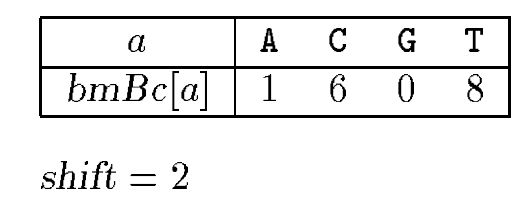
\includegraphics[width=10cm]{Images/2026-05-18-10-15-33.png}
\end{center}

Bảng $bmBc$ được sử dụng bởi thuật toán Tuned Boyer-Moore.

\textbf{Pha tìm kiếm:}

Lần 1:

\begin{center}
    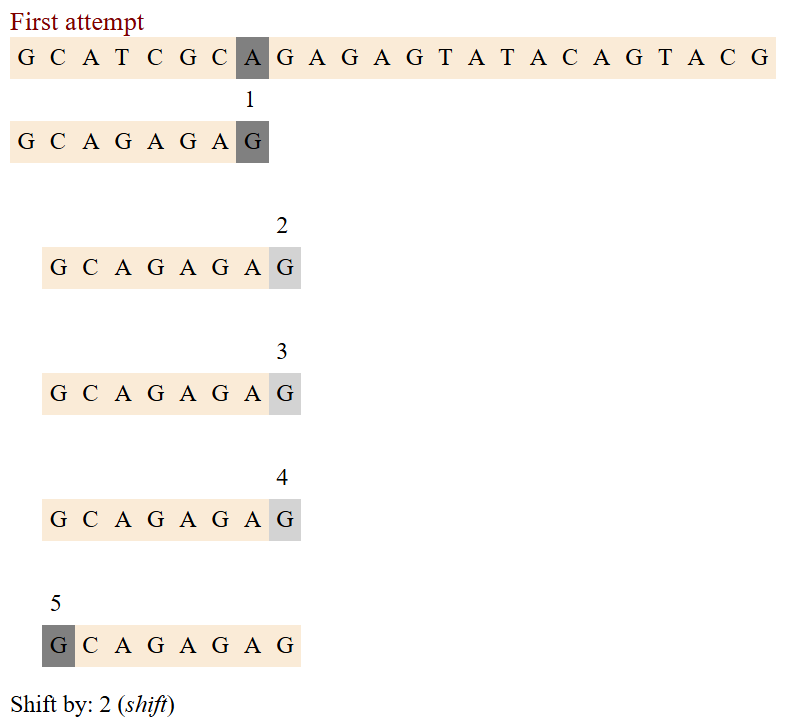
\includegraphics[width=15cm]{Images/2026-05-18-10-16-24.png}
\end{center}

Lần 2:

\begin{center}
    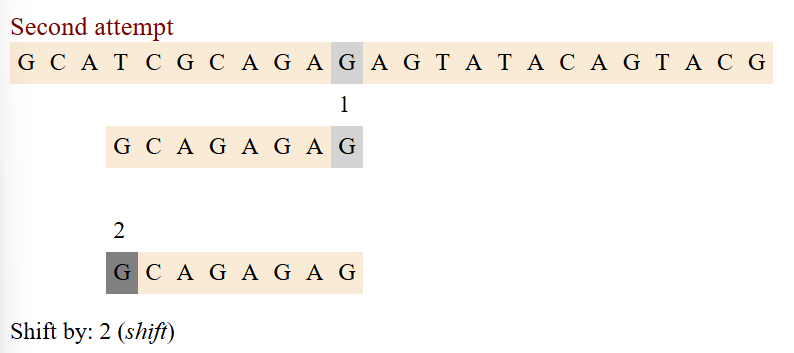
\includegraphics[width=15cm]{Images/2026-05-18-10-16-42.png}
\end{center}

Lần 3:

\begin{center}
    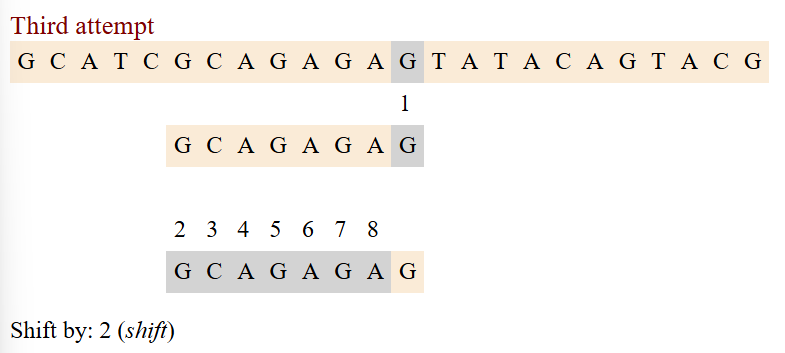
\includegraphics[width=15cm]{Images/2026-05-18-10-17-00.png}
\end{center}

Lần 4:

\begin{center}
    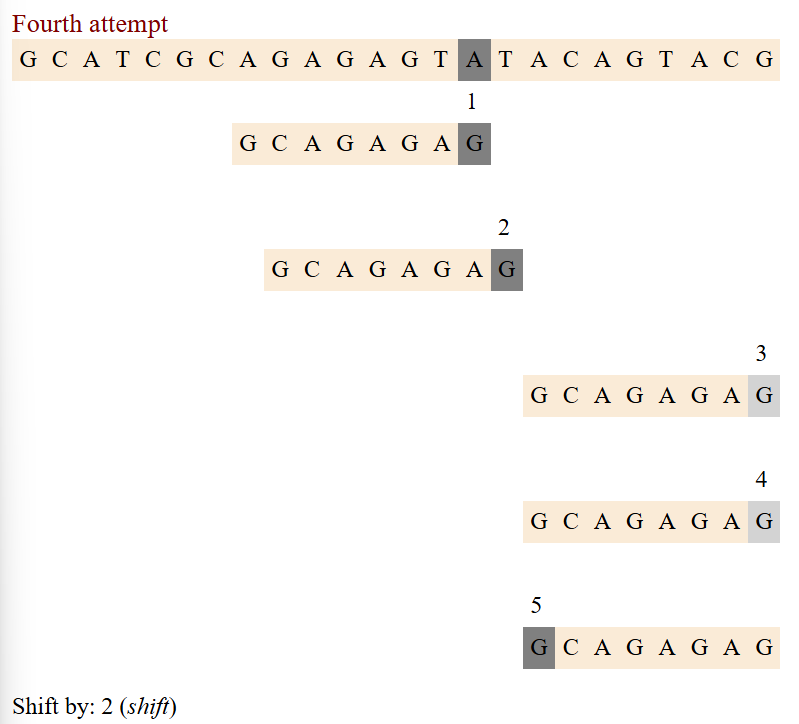
\includegraphics[width=15cm]{Images/2026-05-18-10-17-23.png}
\end{center}

Thuật toán Tuned Boyer Moore thực hiện 10 phép so sánh ký tự trong ví dụ trên.